\documentclass{article}

% Setting up the page
\usepackage[english]{babel}
\usepackage[utf8]{inputenc}
\usepackage{lmodern}
\usepackage{fullpage}

% Writing mathematics, algorithms and code
\usepackage{mathtools}
\usepackage{amsmath}
\usepackage{amssymb}
\usepackage{algpseudocode}
\usepackage{algorithmicx}
\usepackage{algorithm}
%\usepackage{minted}

% Importing images, tables and referencing
\usepackage{graphicx}
%\usepackage{hyperref}
\usepackage{booktabs}
\usepackage{float}

% For indexing sections, etc.
\usepackage{amsthm}
\theoremstyle{definition}
\newtheorem{definition}{Definition}[section]
\newtheorem{theorem}{Theorem}
\newtheorem{example}{Example}
\newtheorem*{remark}{Remark}

% Bibliography
\usepackage[backend=bibtex]{biblatex}
\addbibresource{thesis.bib}


\title{Comparing initialisation processes for the \(k\)-modes algorithm, and an 
	alternative process utilising the hospital-resident assignment problem}
\author{Henry Wilde}

\begin{document}
\maketitle


\section{The \(k\)-modes algorithm}\label{section:kmodes}
The \(k\)-modes algorithm is a part of the family of clustering algorithms known 
as `prototype-based clustering', and is an extension of the \(k\)-means 
algorithm for categorical data as set out in~\cite{Huang98}. This work will 
outline the key differences between the two algorithms, and then aim to 
examine how the initial cluster selection process has an impact on the 
efficiency and quality of the \(k\)-modes algorithm.\\


\subsection{Notation}\label{subsection:notation}

We will use the following notation throughout this work to describe our data 
set, points, clusters and representative points:

\begin{itemize}
    \item Our dataset has \(N\) elements and is denoted by \textbf{X}.
    \item \textbf{X} is described by a set of \(m \in \mathbb{Z}_+\) attributes 
        \(\textbf{A} = \{A_1, \ldots, A_m\}\).
    \item Each attribute \(A_j\) draws its values from a set \(dom(A_j) = 
        \{a_1^{(j)}, \ldots, a_{d_j}^{(j)}\}\) where \(d_j = |dom(A_j)| \in 
        \mathbb{Z}_+\) is sometimes used as shorthand.
    \item We write each data point \(X^{(i)}\) as an \(m\)-dimensional vector:
	\[
		X^{(i)} = [A_1 = x_1^{(i)}, A_2 = x_2^{(i)}, \ldots, A_m = 
				x_m^{(i)}], \ \ i=1, \ldots, N
	\]
        where \(x_j^{(i)}\) is the value of the \(j^{th}\) attribute of the
        \(i^{th}\) data point, \(X^{(i)}\).
	\item Prototype-based clustering algorithms partition the elements of 
        \(\textbf{X}\) into \(k\) distinct sets (clusters) denoted by \(C_1, 
        \ldots, C_k\), where \(k \in \mathbb{Z}_+\) is a pre-determined, fixed 
        integer such that \(k \le N\). That is:
	\[
		C_1, \ldots, C_k \text{ are such that } \bigcup_{l=1}^k C_l = 
		\textbf{X} \quad \text{and} \quad C_l \cap C_t = \emptyset 
		\text{ for all } l \ne t
	\]
    \item Each cluster \(C_l\) has associated with it a representative point 
		(see: Section~\ref{subsection:rep-points}) which we denote by 
        \(\mu^{(l)}~=~[\mu_1^{(l)},~\ldots,~\mu_m^{(l)}]\).
\end{itemize}


\subsection{Dissimilarity measure}\label{subsection:dissim}

An immediate difference between the \(k\)-means and \(k\)-modes algorithms is 
that they deal with different types of data, and so the metric used to define 
the distance between two points in our space must be different. With 
\(k\)-means, where the data has all-numeric attributes, Euclidean distance is 
often used. However, we do not have this sense of distance with categorical 
data. Instead, we utilise a dissimilarity measure - defined below - as our 
metric. It can be easily checked that this is indeed a distance measure.\\

\begin{definition}\label{def:dissim}
	Let $\textbf{X}$ be a data set and consider $X^{(a)}, X^{(b)} \in 
    \textbf{X}$. We define the \emph{dissimilarity} between $X^{(a)}$ and 
    $X^{(b)}$, denoted by \(d(X^{(a)}, X^{(b)})\), to be:
	\[
	d(X^{(a)}, X^{(b)}) = \sum_{j=1}^{m} \delta(x_j^{(a)}, x_j^{(b)}) \quad
	\text{where} \quad \delta(x, y) = \begin{cases}
                                        0, & x = y \\
					                    1, & \text{otherwise}
					                  \end{cases}
	\]

    In other words, the dissimilarity between two points is the number of
    attributes where they are not the same.
\end{definition}


\begin{example}
    Throughout this paper, we will make use of a small numerical example to aid 
    our understanding of concepts. The dataset we will use is available online 
    at~\url{https://www.kaggle.com/uciml/zoo-animal-classification/data}.\\

    This dataset is built for the classification of zoo animals. There are 101
    instances, described by 16 (mostly binary) attributes, their name and a 
    class label indicating the type of animal they are. The first five rows of 
    the dataset are given in Table~\ref{tab:zoo-head}.\\
    
    \begin{table}[h]
    \resizebox{\textwidth}{!}{%
        \centering
        \begin{tabular}{llllllllllllllllllr}
\toprule
{} & animal\_name &   hair &  feathers &   eggs &   milk &  airborne &  aquatic &  predator &  toothed &  backbone &  breathes &  venomous &   fins &  legs &   tail &  domestic &  catsize &  class\_type \\
\midrule
0 &    aardvark &   True &     False &  False &   True &     False &    False &      True &     True &      True &      True &     False &  False &  Four &  False &     False &     True &           1 \\
1 &    antelope &   True &     False &  False &   True &     False &    False &     False &     True &      True &      True &     False &  False &  Four &   True &     False &     True &           1 \\
2 &        bass &  False &     False &   True &  False &     False &     True &      True &     True &      True &     False &     False &   True &  None &   True &     False &    False &           4 \\
3 &        bear &   True &     False &  False &   True &     False &    False &      True &     True &      True &      True &     False &  False &  Four &  False &     False &     True &           1 \\
4 &        boar &   True &     False &  False &   True &     False &    False &      True &     True &      True &      True &     False &  False &  Four &   True &     False &     True &           1 \\
\bottomrule
\end{tabular}

    }
    \caption{The head of the zoo animal dataset}
    \label{tab:zoo-head}
    \end{table}
\end{example}

\subsection{Representative points}\label{subsection:rep-points}

Now that we have defined a metric on our space, we can turn our attention to 
what we mean by the representative point \(\mu^{(l)}\) of a cluster \(C_l\). In 
\(k\)-means, we call \(\mu^{(l)}\) a `centroid' and define it to be the average 
of all points \(X^{(i)} \in C_l\) by Euclidean distance. With categorical data, 
we use our revised distance measure from Definition~\ref{def:dissim} to specify 
a representative point. We call such a point a mode of \textbf{X}.\\

\begin{definition}\label{def:mode}
    We define a \emph{mode} of our set \textbf{X} to be any vector \(\mu = 
    [\mu_1, \ldots, \mu_m]\) that minimises:
	
    \begin{equation}
		D(\textbf{X}, \mu) = \sum_{i=1}^{n} d(X_i, \mu)
	\end{equation}
	
    Note that \(\mu\) is not necessarily in \textbf{X}. We call such a mode a 
    \emph{virtual mode}.
\end{definition}

\begin{definition}\label{def:rel-freq}
    Let \textbf{X} be a dataset with attributes \(A_1, \ldots, A_m\). Then we
    denote by \(n(a_s^{(j)})\) the \emph{frequency} of the \(s^{th}\) category 
    \(a_s^{(j)}\) of \(A_j\) in \textbf{X}. That is, 
	
    \[
	    n(a_s^{(j)}) := |{\{X^{(i)} \in \textbf{X}: x_j^{(i)} = a_s^{(j)}\}}|
	\]
	
    We call \(\frac{n(a_s^{(j)})}{N}\) the \emph{relative frequency} of category 
    \(a_s^{(j)}\) in \textbf{X}.
\end{definition}

\begin{remark}
    Note that we have \(1 \le n(a_s^{(j)}) \le N\) for all \(s\) and \(j = 1, 
    \ldots, m\).\\
\end{remark}

\begin{theorem}\label{theorem:1}
    Consider a dataset \textbf{X} and some \(X^{(i)} \in \textbf{X}\). Then:
	
    \[
	    D(\textbf{X}, X^{(i)}) \text{ is minimised } \iff n(x_j^{(i)}) \geq 
	    n(a_s^{(j)}) \text{ for all } s \text{ and } j = 1, \ldots, m 
	\]
\end{theorem}
A proof of this theorem can be found in the Appendix of~\cite{Huang98}.\\


\subsection{The cost function}\label{subsection:cost}

We can use Definitions~\ref{def:dissim}~\&~\ref{def:mode} to determine a cost 
function for our algorithm. Let \(\bar{\mu} = \{\mu^{(1)}, \ldots, \mu^{(k)}\}\) 
be a set of \(k\) modes of \textbf{X}, and let \(W = (w_{i,l})\) be an \(n 
\times k\) matrix such that:

\[ 
    w_{i,l} = \begin{cases}
                1, & X^{(i)} \in C_l \\
                0, & \text{otherwise}
              \end{cases}
\]\\

Then we define our \emph{cost function} to be the summed within-cluster 
dissimilarity:

\begin{equation}
    \text{Cost}(W, \bar{\mu}) = \sum_{l=1}^{k} \sum_{i=1}^{n} 
                                \sum_{j=1}^{m} w_{i,l} 
                                \delta(x_{i,j}, \mu_{l,j})
\end{equation}


\subsection{The \(k\)-modes algorithm}\label{subsection:kmodes}

Below is a practical implementation of the \(k\)-modes algorithm \cite{Huang98}:

\begin{algorithm}[H]
    \caption{\(k\)-modes}\label{alg:kmodes}
	\begin{algorithmic}[0] 
        \State \(\bar{\mu} \gets \emptyset\)
        \For {\(l \in \{1, \ldots, k\}\)}
            \State \(C_l \gets \emptyset\)
		\EndFor
        \State Select \(k\) initial modes, \(\mu^{(1)}, \ldots, \mu^{(k)}\).
        \State \(\bar{\mu} \gets \{\mu^{(1)}, \ldots, \mu^{(k)}\}\)
        \For {\(X_i \in \textbf{X}\)}
            \State Select \(l^* \text{ that satisfies } \displaystyle{d(X^{(i)}, 
                \mu^{(l^*)}) = \min_{1 \le l \le m} \{d(X^{(i)}, \mu^{(l)})\}}\)
            \State \(C_{j^*} \gets C_{j^*} \cup \{X^{(i)}\}\)
            \State Update \(\mu^{(l^*)}\)
		\EndFor
		\Repeat
            \For {\(X^{(i)} \in \textbf{X}\)}
                \For {\(\mu^{(l)} \in \bar{\mu}\)}
                    \State Calculate \(d(X^{(i)}, \mu^{(l)})\)
				\EndFor
                \If {\(d(X^{(i)}, \mu^{(l^*)}) > d(X^{(i)}, \mu^{(l')}) \text{ 
                    for some } l' \ne l^*\)}
                    \State \(C_{l^*} \gets C_{l^*} \setminus \{X^{(i)}\}\)
                    \State \(C_{l'} \gets C_{l'} \cup \{X^{(i)}\}\)
                    \State Update both \(\mu^{(l^*)} \text{ and } \mu^{(j')}\)
				\EndIf
			\EndFor
		\Until {No point changes cluster after a full cycle through \textbf{X}}
	\end{algorithmic}
\end{algorithm}

\begin{remark}
    The processes by which the \(k\) initial modes are selected are detailed in 
    Sections~\ref{section:init}~\&~\ref{section:new-method}.
\end{remark}




\section{Initialisation processes}\label{section:init}
From the literature surrounding this topic, it has been established that the 
initial choice of clusters impacts the final solution of the \(k\)-modes
algorithm~\cite{Huang98}~\cite{Cao09}. While some works attempt to improve the 
quality of \(k\)-modes and similar algorithms by considering an alternative 
dissimilarity measure~\cite{Ng07}, this work will examine the way in which these
\(k\) initial representative points are chosen. Two established methods of 
selecting these initial points are described in
Sections~\ref{subsec:huang}~\&~\ref{subsec:cao}.\\


\subsection{Huang's method}\label{subsec:huang}

In the standard form of the \(k\)-modes algorithm, the \(k\) initial modes are 
chosen at random from \textbf{X}. Below is an alternative method of selecting
these modes that forces some diversity between them, as described 
in~\cite{Huang98}. Here, we consider two sets of modes, \(\tilde{\mu}\) and
\(\bar{\mu}\). The former acts as a placeholder set of modes, whereas the latter
is the set of modes to go on to be used by the \(k\)-modes algorithm.\\

\begin{algorithm}[H]
\caption{Huang's method}\label{alg:huang}
    \begin{algorithmic}[0]
        \State{\textbf{Input:} a dataset \textbf{X}, with attribute sets \(A_1,
        \ldots, A_m\), and a number of modes to find \(k\)}
        \State{\textbf{Output:} a set of \(k\) initial modes \(\bar{\mu}\)}
        \\
        \State{\(\tilde{\mu} \gets \emptyset\)}\Comment{Initialisation step}
        \State{\(\bar{\mu} \gets \emptyset\)}
        \For{\(j = 1, \ldots, m\)}
            \For{\(s = 1, \ldots, d_j\)}
                \State{Calculate the relative frequency of each attribute value:
                    \(\frac{n(a_s^{(j)})}{N}\).}
	        \EndFor
        \EndFor
        \\
        \For{\(l = 1, \ldots, k\)}\Comment{Distribute most common attribute 
        values}
            \For{\(j = 1, \ldots, m\)}
            \State{Sample \(a_{s^*}^{(j)}\) from \(A_j\) by considering the 
                relative frequencies of the elements of \(A_j\) as a probability
                distribution.}
                \State{\(\mu_j^{(l)} \gets a_{s^*}^{(j)}\)}
	        \EndFor
            \State{\(\tilde{\mu} \gets \tilde{\mu} \cup \{\mu^{(l)}\}\)}
	    \EndFor
        \\
        \For{\(\mu \in \tilde{\mu}\)}\Comment{Replace with points in dataset to
        avoid empty clusters}
            \State{Select \(X^{(i^*)} \in \textbf{X}\) such that: 
                \[
                    X^{(i^*)} = \argmin_{1 \leq i \leq N} \left\{ d(X^{(i)}, 
                    \mu): \ X^{(i^*)} \neq \mu'  \ \forall \mu' \in 
                    \bar{\mu}\right\}
                \]
            }
            \State{\(\bar{\mu} \gets \bar{\mu} \cup \left\{X^{(i^*)}\right\}\)}
        \EndFor
    \end{algorithmic}
\end{algorithm} 

In the original statement of Huang's method~\cite{Huang98}, the algorithm states
that the most frequent categories should be assigned `equally' to the \(k\) 
initial modes. How the categories should be distributed `equally' is not 
well-defined or easily seen from the example given. This ambiguity in the 
definition of Huang's method means that a probabilistic element must be 
introduced, and unless seeded pseudo-random numbers are used, computer-generated results are not necessarily reproducible.\\

In Section~\ref{sec:results}, an implementation of the \(k\)-modes algorithm 
(written in Python) is used to compare the quality of the initialisation 
processes discussed throughout this piece of work when applied to a collection 
of datasets. That implementation distributes the attribute values by taking a
sample from each attribute domain (with replacement) according to the 
probability distribution formed by the relative frequencies of the attribute
values, as is described in Algorithm~\ref{alg:huang}. In our examples, we will
assign the categories to our initial modes in the same way.\\

\begin{example}\label{ex:huang}
    Consider the zoo animal dataset. We will now find a set of initial modes for
    the \(k\)-modes algorithm using Huang's method. For the sake of this
    example, we will let \(k = 7\) as there are \(7\) classes. Please be advised
    that this may not be the optimal value for \(k\).\\
    
    We begin by calculating the frequencies and relative frequencies of our 
    attributes' values, which are stored in 
    Tables~\ref{tab:freq}~\&~\ref{tab:rel-freq}, respectively.

    \begin{table}[h]
    \resizebox{\textwidth}{!}{%
        \begin{tabular}{lrrrrrrrrrrrrrrrr}
\toprule
{} &  hair &  feathers &  eggs &  milk &  airborne &  aquatic &  predator &  toothed &  backbone &  breathes &  venomous &  fins &  legs &  tail &  domestic &  catsize \\
\midrule
False &    58 &        81 &    42 &    60 &        77 &       65 &        45 &       40 &        18 &        21 &        93 &    84 &     0 &    26 &        88 &       57 \\
True  &    43 &        20 &    59 &    41 &        24 &       36 &        56 &       61 &        83 &        80 &         8 &    17 &     0 &    75 &        13 &       44 \\
Four  &     0 &         0 &     0 &     0 &         0 &        0 &         0 &        0 &         0 &         0 &         0 &     0 &    38 &     0 &         0 &        0 \\
Two   &     0 &         0 &     0 &     0 &         0 &        0 &         0 &        0 &         0 &         0 &         0 &     0 &    27 &     0 &         0 &        0 \\
None  &     0 &         0 &     0 &     0 &         0 &        0 &         0 &        0 &         0 &         0 &         0 &     0 &    23 &     0 &         0 &        0 \\
Six   &     0 &         0 &     0 &     0 &         0 &        0 &         0 &        0 &         0 &         0 &         0 &     0 &    10 &     0 &         0 &        0 \\
Eight &     0 &         0 &     0 &     0 &         0 &        0 &         0 &        0 &         0 &         0 &         0 &     0 &     2 &     0 &         0 &        0 \\
Five  &     0 &         0 &     0 &     0 &         0 &        0 &         0 &        0 &         0 &         0 &         0 &     0 &     1 &     0 &         0 &        0 \\
\bottomrule
\end{tabular}

    }
    \caption{Frequency table for attribute values.}\label{tab:freq}
    \end{table}

    Now that we have the frequency distributions for our attributes, we can
    arrange our attribute domains into descending order of frequency:
    
    \begin{equation}
    \begin{aligned}
    \nonumber
    \centering
        dom^*(\text{hair}) = \left[\false, \true\right], \
        dom^*(\text{feathers}) = \left[\false, \true \right], & \ &
        dom^*(\text{eggs}) = \left[\true, \false\right], \
        dom^*(\text{milk}) = \left[\false, \true\right],
        \\
        {} & \vdots & {}
        \\
        dom^*(\text{legs}) = \left[\text{Four, Two, None, Six, Eight, 
        Five}\right], \
        dom^*(\text{tail}) = \left[\true, \false\right], & \ &
        dom^*(\text{domestic}) = \left[\false, \true\right], \
        dom^*(\text{catsize}) = \left[\false, \true\right]
        \\
    \end{aligned}
    \end{equation}

    \begin{table}[h]
    \resizebox{\textwidth}{!}{%
        \begin{tabular}{ccccccccccccccccc}
\toprule
{} &    hair & feathers &    eggs &    milk & airborne & aquatic & predator & toothed & backbone & breathes & venomous &    fins &    legs &    tail & domestic & catsize \\
\midrule
False &  58/101 &   81/101 &  42/101 &  60/101 &   77/101 &  65/101 &   45/101 &  40/101 &   18/101 &   21/101 &   93/101 &  84/101 &       0 &  26/101 &   88/101 &  57/101 \\
True  &  43/101 &   20/101 &  59/101 &  41/101 &   24/101 &  36/101 &   56/101 &  61/101 &   83/101 &   80/101 &    8/101 &  17/101 &       0 &  75/101 &   13/101 &  44/101 \\
Four  &       0 &        0 &       0 &       0 &        0 &       0 &        0 &       0 &        0 &        0 &        0 &       0 &  38/101 &       0 &        0 &       0 \\
Two   &       0 &        0 &       0 &       0 &        0 &       0 &        0 &       0 &        0 &        0 &        0 &       0 &  27/101 &       0 &        0 &       0 \\
None  &       0 &        0 &       0 &       0 &        0 &       0 &        0 &       0 &        0 &        0 &        0 &       0 &  23/101 &       0 &        0 &       0 \\
Six   &       0 &        0 &       0 &       0 &        0 &       0 &        0 &       0 &        0 &        0 &        0 &       0 &  10/101 &       0 &        0 &       0 \\
Eight &       0 &        0 &       0 &       0 &        0 &       0 &        0 &       0 &        0 &        0 &        0 &       0 &   2/101 &       0 &        0 &       0 \\
Five  &       0 &        0 &       0 &       0 &        0 &       0 &        0 &       0 &        0 &        0 &        0 &       0 &   1/101 &       0 &        0 &       0 \\
\bottomrule
\end{tabular}

    }
    \caption{Relative frequency table for attribute values.}\label{tab:rel-freq}
    \end{table}

    Now to find our set of (potentially) virtual modes, \(\bar{\mu}\). For each
    attribute, we will take a sample of size one from the attribute domain
    according to the probability distribution represented in the corresponding
    column of Table~\ref{tab:rel-freq}. The following set of initial modes was 
    obtained by using a short Python script (put in Appendix). It can be easily
    checked that these vectors minimise our summed dissimilarity function
    \(D(\textbf{X}, \mu)\) with value \(101\), thus satisfying 
    Theorem~\ref{thm:1}.

    \begin{equation}
    \nonumber
    \begin{aligned}
        \bar{\mu} = \ \{ & \mu^{(1)} = \left[\false, \ \false, \ \true, \ 
        \false, \ \false, \ \true, \ \false, \ \true, \ \true, \ \true, \ 
        \false, \ \false, \ \text{Two}, \ \true, \ \false, \ \false\right],
        \\
        {} & \mu^{(2)} = \left[\false, \ \true, \ \true, \ \true, \ \true, \
        \true, \ \true, \ \true, \ \false, \ \true, \ \false, \ \true, \
        \text{Two}, \ \true, \ \false, \ \true\right],
        \\
        {} & \mu^{(3)} = \left[\false, \ \false, \ \false, \ \true, \ \false, \
        \false, \ \true, \ \true, \ \true, \ \true, \ \false, \false, 
        \text{None}, \ \true, \ \false, \ \false\right],
        \\
        {} & \mu^{(4)} = \left[\false, \ \false, \ \true, \ \false, \ \true, \
        \false, \ \false, \ \false, \ \true, \ \true, \ \false, \false, \
        \text{Four}, \ \false, \ \false, \false\right],
        \\
        {} & \mu^{(5)} = \left[\false, \ \false, \ \true, \ \false, \ \true, \
        \false, \ \true, \ \true, \ \true, \ \true, \ \false, \ \false, \
        \text{Four}, \ \false, \false, \false\right],
        \\
        {} & \mu^{(6)} = \left[\false, \ \false, \ \false, \ \true, \ \false, \
        \false, \ \true, \ \false, \ \true, \ \true, \ \false, \ \false, \
        \text{Four}, \ \true, \ \false, \ \false\right],
        \\
        {} & \mu^{(7)} = \left[\true, \ \false, \ \true, \ \false, \ \false, \
        \false, \ \true, \ \true, \ \true, \ \true, \ \false, \ \false, \ 
        \text{Four}, \ \true, \ \false, \ \true\right]\}\\
    \end{aligned}
    \end{equation}

    Finally, we take each element of \(\bar{\mu}\) in turn and replace it with
    the most similar point in our dataset such that no point is used twice.
    These \(k\) modes are given in Table~\ref{tab:huang-modes}.
    We also stipulate that if there is more than one entry in the set with the 
    same attributes as another (for instance, aardvark and bear are identical in
    this setting) that only one of these entries may be used as a replacement 
    for one of our virtual modes.\\

    \begin{table}[h]
    \resizebox{\textwidth}{!}{%
        \begin{tabular}{llllllllllllllllllr}
\toprule
{} & animal\_name &   hair &  feathers &   eggs &   milk &  airborne &  aquatic &  predator &  toothed &  backbone &  breathes &  venomous &   fins &   legs &   tail &  domestic &  catsize &  class\_type \\
\midrule
92  &     tuatara &  False &     False &   True &  False &     False &    False &      True &     True &      True &      True &     False &  False &   Four &   True &     False &    False &           3 \\
81  &    slowworm &  False &     False &   True &  False &     False &    False &      True &     True &      True &      True &     False &  False &   None &   True &     False &    False &           3 \\
53  &        newt &  False &     False &   True &  False &     False &     True &      True &     True &      True &      True &     False &  False &   Four &   True &     False &    False &           5 \\
91  &    tortoise &  False &     False &   True &  False &     False &    False &     False &    False &      True &      True &     False &  False &   Four &   True &     False &     True &           3 \\
55  &     opossum &   True &     False &  False &   True &     False &    False &      True &     True &      True &      True &     False &  False &   Four &   True &     False &    False &           1 \\
50  &        mole &   True &     False &  False &   True &     False &    False &      True &     True &      True &      True &     False &  False &   Four &   True &     False &    False &           1 \\
95  &        vole &   True &     False &  False &   True &     False &    False &     False &     True &      True &      True &     False &  False &   Four &   True &     False &    False &           1 \\
37  &        hare &   True &     False &  False &   True &     False &    False &     False &     True &      True &      True &     False &  False &   Four &   True &     False &    False &           1 \\
51  &    mongoose &   True &     False &  False &   True &     False &    False &      True &     True &      True &      True &     False &  False &   Four &   True &     False &     True &           1 \\
65  &     polecat &   True &     False &  False &   True &     False &    False &      True &     True &      True &      True &     False &  False &   Four &   True &     False &     True &           1 \\
70  &     raccoon &   True &     False &  False &   True &     False &    False &      True &     True &      True &      True &     False &  False &   Four &   True &     False &     True &           1 \\
48  &        lynx &   True &     False &  False &   True &     False &    False &      True &     True &      True &      True &     False &  False &   Four &   True &     False &     True &           1 \\
46  &        lion &   True &     False &  False &   True &     False &    False &      True &     True &      True &      True &     False &  False &   Four &   True &     False &     True &           1 \\
45  &     leopard &   True &     False &  False &   True &     False &    False &      True &     True &      True &      True &     False &  False &   Four &   True &     False &     True &           1 \\
68  &        puma &   True &     False &  False &   True &     False &    False &      True &     True &      True &      True &     False &  False &   Four &   True &     False &     True &           1 \\
99  &        wolf &   True &     False &  False &   True &     False &    False &      True &     True &      True &      True &     False &  False &   Four &   True &     False &     True &           1 \\
11  &     cheetah &   True &     False &  False &   True &     False &    False &      True &     True &      True &      True &     False &  False &   Four &   True &     False &     True &           1 \\
5   &        boar &   True &     False &  False &   True &     False &    False &      True &     True &      True &      True &     False &  False &   Four &   True &     False &     True &           1 \\
85  &    squirrel &   True &     False &  False &   True &     False &    False &     False &     True &      True &      True &     False &  False &    Two &   True &     False &    False &           1 \\
29  &     giraffe &   True &     False &  False &   True &     False &    False &     False &     True &      True &      True &     False &  False &   Four &   True &     False &     True &           1 \\
2   &    antelope &   True &     False &  False &   True &     False &    False &     False &     True &      True &      True &     False &  False &   Four &   True &     False &     True &           1 \\
23  &    elephant &   True &     False &  False &   True &     False &    False &     False &     True &      True &      True &     False &  False &   Four &   True &     False &     True &           1 \\
18  &        deer &   True &     False &  False &   True &     False &    False &     False &     True &      True &      True &     False &  False &   Four &   True &     False &     True &           1 \\
56  &        oryx &   True &     False &  False &   True &     False &    False &     False &     True &      True &      True &     False &  False &   Four &   True &     False &     True &           1 \\
6   &     buffalo &   True &     False &  False &   True &     False &    False &     False &     True &      True &      True &     False &  False &   Four &   True &     False &     True &           1 \\
26  &        frog &  False &     False &   True &  False &     False &     True &      True &     True &      True &      True &     False &  False &   Four &  False &     False &    False &           5 \\
97  &     wallaby &   True &     False &  False &   True &     False &    False &     False &     True &      True &      True &     False &  False &    Two &   True &     False &     True &           1 \\
90  &        toad &  False &     False &   True &  False &     False &     True &     False &     True &      True &      True &     False &  False &   Four &  False &     False &    False &           5 \\
42  &        kiwi &  False &      True &   True &  False &     False &    False &      True &    False &      True &      True &     False &  False &    Two &   True &     False &    False &           2 \\
49  &        mink &   True &     False &  False &   True &     False &     True &      True &     True &      True &      True &     False &  False &   Four &   True &     False &     True &           1 \\
64  &    platypus &   True &     False &   True &   True &     False &     True &      True &    False &      True &      True &     False &  False &   Four &   True &     False &     True &           1 \\
63  &    pitviper &  False &     False &   True &  False &     False &    False &      True &     True &      True &      True &      True &  False &   None &   True &     False &    False &           3 \\
72  &        rhea &  False &      True &   True &  False &     False &    False &      True &    False &      True &      True &     False &  False &    Two &   True &     False &     True &           2 \\
4   &        bear &   True &     False &  False &   True &     False &    False &      True &     True &      True &      True &     False &  False &   Four &  False &     False &     True &           1 \\
1   &    aardvark &   True &     False &  False &   True &     False &    False &      True &     True &      True &      True &     False &  False &   Four &  False &     False &     True &           1 \\
57  &     ostrich &  False &      True &   True &  False &     False &    False &     False &    False &      True &      True &     False &  False &    Two &   True &     False &     True &           2 \\
94  &     vampire &   True &     False &  False &   True &      True &    False &     False &     True &      True &      True &     False &  False &    Two &   True &     False &    False &           1 \\
28  &    fruitbat &   True &     False &  False &   True &      True &    False &     False &     True &      True &      True &     False &  False &    Two &   True &     False &    False &           1 \\
33  &     gorilla &   True &     False &  False &   True &     False &    False &     False &     True &      True &      True &     False &  False &    Two &  False &     False &     True &           1 \\
59  &     penguin &  False &      True &   True &  False &     False &     True &      True &    False &      True &      True &     False &  False &    Two &   True &     False &     True &           2 \\
36  &     hamster &   True &     False &  False &   True &     False &    False &     False &     True &      True &      True &     False &  False &   Four &   True &      True &    False &           1 \\
69  &    pussycat &   True &     False &  False &   True &     False &    False &      True &     True &      True &      True &     False &  False &   Four &   True &      True &     True &           1 \\
38  &        hawk &  False &      True &   True &  False &      True &    False &      True &    False &      True &      True &     False &  False &    Two &   True &     False &    False &           2 \\
17  &        crow &  False &      True &   True &  False &      True &    False &      True &    False &      True &      True &     False &  False &    Two &   True &     False &    False &           2 \\
7   &        calf &   True &     False &  False &   True &     False &    False &     False &     True &      True &      True &     False &  False &   Four &   True &      True &     True &           1 \\
32  &        goat &   True &     False &  False &   True &     False &    False &     False &     True &      True &      True &     False &  False &   Four &   True &      True &     True &           1 \\
66  &        pony &   True &     False &  False &   True &     False &    False &     False &     True &      True &      True &     False &  False &   Four &   True &      True &     True &           1 \\
71  &    reindeer &   True &     False &  False &   True &     False &    False &     False &     True &      True &      True &     False &  False &   Four &   True &      True &     True &           1 \\
101 &        wren &  False &      True &   True &  False &      True &    False &     False &    False &      True &      True &     False &  False &    Two &   True &     False &    False &           2 \\
44  &        lark &  False &      True &   True &  False &      True &    False &     False &    False &      True &      True &     False &  False &    Two &   True &     False &    False &           2 \\
60  &    pheasant &  False &      True &   True &  False &      True &    False &     False &    False &      True &      True &     False &  False &    Two &   True &     False &    False &           2 \\
84  &     sparrow &  False &      True &   True &  False &      True &    False &     False &    False &      True &      True &     False &  False &    Two &   True &     False &    False &           2 \\
96  &     vulture &  False &      True &   True &  False &      True &    False &      True &    False &      True &      True &     False &  False &    Two &   True &     False &     True &           2 \\
20  &     dolphin &  False &     False &  False &   True &     False &     True &      True &     True &      True &      True &     False &   True &   None &   True &     False &     True &           1 \\
67  &    porpoise &  False &     False &  False &   True &     False &     True &      True &     True &      True &      True &     False &   True &   None &   True &     False &     True &           1 \\
100 &        worm &  False &     False &   True &  False &     False &    False &     False &    False &     False &      True &     False &  False &   None &  False &     False &    False &           7 \\
82  &        slug &  False &     False &   True &  False &     False &    False &     False &    False &     False &      True &     False &  False &   None &  False &     False &    False &           7 \\
27  &        frog &  False &     False &   True &  False &     False &     True &      True &     True &      True &      True &      True &  False &   Four &  False &     False &    False &           5 \\
9   &     catfish &  False &     False &   True &  False &     False &     True &      True &     True &      True &     False &     False &   True &   None &   True &     False &    False &           4 \\
39  &     herring &  False &     False &   True &  False &     False &     True &      True &     True &      True &     False &     False &   True &   None &   True &     False &    False &           4 \\
13  &        chub &  False &     False &   True &  False &     False &     True &      True &     True &      True &     False &     False &   True &   None &   True &     False &    False &           4 \\
62  &     piranha &  False &     False &   True &  False &     False &     True &      True &     True &      True &     False &     False &   True &   None &   True &     False &    False &           4 \\
24  &    flamingo &  False &      True &   True &  False &      True &    False &     False &    False &      True &      True &     False &  False &    Two &   True &     False &     True &           2 \\
3   &        bass &  False &     False &   True &  False &     False &     True &      True &     True &      True &     False &     False &   True &   None &   True &     False &    False &           4 \\
76  &     sealion &   True &     False &  False &   True &     False &     True &      True &     True &      True &      True &     False &   True &    Two &   True &     False &     True &           1 \\
25  &        flea &  False &     False &   True &  False &     False &    False &     False &    False &     False &      True &     False &  False &    Six &  False &     False &    False &           6 \\
89  &     termite &  False &     False &   True &  False &     False &    False &     False &    False &     False &      True &     False &  False &    Six &  False &     False &    False &           6 \\
79  &     skimmer &  False &      True &   True &  False &      True &     True &      True &    False &      True &      True &     False &  False &    Two &   True &     False &    False &           2 \\
80  &        skua &  False &      True &   True &  False &      True &     True &      True &    False &      True &      True &     False &  False &    Two &   True &     False &    False &           2 \\
34  &        gull &  False &      True &   True &  False &      True &     True &      True &    False &      True &      True &     False &  False &    Two &   True &     False &    False &           2 \\
74  &    seahorse &  False &     False &   True &  False &     False &     True &     False &     True &      True &     False &     False &   True &   None &   True &     False &    False &           4 \\
83  &        sole &  False &     False &   True &  False &     False &     True &     False &     True &      True &     False &     False &   True &   None &   True &     False &    False &           4 \\
35  &     haddock &  False &     False &   True &  False &     False &     True &     False &     True &      True &     False &     False &   True &   None &   True &     False &    False &           4 \\
93  &        tuna &  False &     False &   True &  False &     False &     True &      True &     True &      True &     False &     False &   True &   None &   True &     False &     True &           4 \\
19  &     dogfish &  False &     False &   True &  False &     False &     True &      True &     True &      True &     False &     False &   True &   None &   True &     False &     True &           4 \\
61  &        pike &  False &     False &   True &  False &     False &     True &      True &     True &      True &     False &     False &   True &   None &   True &     False &     True &           4 \\
22  &        duck &  False &      True &   True &  False &      True &     True &     False &    False &      True &      True &     False &  False &    Two &   True &     False &    False &           2 \\
10  &        cavy &   True &     False &  False &   True &     False &    False &     False &     True &      True &      True &     False &  False &   Four &  False &      True &    False &           1 \\
30  &        girl &   True &     False &  False &   True &     False &    False &      True &     True &      True &      True &     False &  False &    Two &  False &      True &     True &           1 \\
88  &        swan &  False &      True &   True &  False &      True &     True &     False &    False &      True &      True &     False &  False &    Two &   True &     False &     True &           2 \\
77  &    seasnake &  False &     False &  False &  False &     False &     True &      True &     True &      True &     False &      True &  False &   None &   True &     False &    False &           3 \\
14  &        clam &  False &     False &   True &  False &     False &    False &      True &    False &     False &     False &     False &  False &   None &  False &     False &    False &           7 \\
43  &    ladybird &  False &     False &   True &  False &      True &    False &      True &    False &     False &      True &     False &  False &    Six &  False &     False &    False &           6 \\
15  &        crab &  False &     False &   True &  False &     False &     True &      True &    False &     False &     False &     False &  False &   Four &  False &     False &    False &           7 \\
73  &    scorpion &  False &     False &  False &  False &     False &    False &      True &    False &     False &      True &      True &  False &  Eight &   True &     False &    False &           7 \\
75  &        seal &   True &     False &  False &   True &     False &     True &      True &     True &      True &      True &     False &   True &   None &  False &     False &     True &           1 \\
31  &        gnat &  False &     False &   True &  False &      True &    False &     False &    False &     False &      True &     False &  False &    Six &  False &     False &    False &           6 \\
12  &     chicken &  False &      True &   True &  False &      True &    False &     False &    False &      True &      True &     False &  False &    Two &   True &      True &    False &           2 \\
58  &    parakeet &  False &      True &   True &  False &      True &    False &     False &    False &      True &      True &     False &  False &    Two &   True &      True &    False &           2 \\
21  &        dove &  False &      True &   True &  False &      True &    False &     False &    False &      True &      True &     False &  False &    Two &   True &      True &    False &           2 \\
52  &        moth &   True &     False &   True &  False &      True &    False &     False &    False &     False &      True &     False &  False &    Six &  False &     False &    False &           6 \\
41  &    housefly &   True &     False &   True &  False &      True &    False &     False &    False &     False &      True &     False &  False &    Six &  False &     False &    False &           6 \\
47  &     lobster &  False &     False &   True &  False &     False &     True &      True &    False &     False &     False &     False &  False &    Six &  False &     False &    False &           7 \\
16  &    crayfish &  False &     False &   True &  False &     False &     True &      True &    False &     False &     False &     False &  False &    Six &  False &     False &    False &           7 \\
8   &        carp &  False &     False &   True &  False &     False &     True &     False &     True &      True &     False &     False &   True &   None &   True &      True &    False &           4 \\
86  &    starfish &  False &     False &   True &  False &     False &     True &      True &    False &     False &     False &     False &  False &   Five &  False &     False &    False &           7 \\
87  &    stingray &  False &     False &   True &  False &     False &     True &      True &     True &      True &     False &      True &   True &   None &   True &     False &     True &           4 \\
54  &     octopus &  False &     False &   True &  False &     False &     True &      True &    False &     False &     False &     False &  False &  Eight &  False &     False &     True &           7 \\
78  &     seawasp &  False &     False &   True &  False &     False &     True &      True &    False &     False &     False &      True &  False &   None &  False &     False &    False &           7 \\
98  &        wasp &   True &     False &   True &  False &      True &    False &     False &    False &     False &      True &      True &  False &    Six &  False &     False &    False &           6 \\
40  &    honeybee &   True &     False &   True &  False &      True &    False &     False &    False &     False &      True &      True &  False &    Six &  False &      True &    False &           6 \\
\bottomrule
\end{tabular}

    }
    \caption{The \(7\) initial modes found by Huang's
    method.}\label{tab:huang-modes}
    \end{table}
\end{example}

\subsection{Cao's method}\label{subsec:cao}

Cao's method selects representative points by the average density of a point in
the dataset. As will be seen in the following definition, this average density 
is in fact the average relative frequency of all the attribute values of that 
point. This method is considered deterministic as there is no probabilistic 
element - unlike the standard or Huang's method - and so results are completely
reproducible.\\

\begin{definition}\label{def:density}	
    Consider a data set \(\textbf{X}\) with attribute set \(\textbf{A} = 
    \{A_1, \ldots, A_m\}\). Then the \emph{average density} of any point 
    \(X_i \in \textbf{X}\) with respect to \(\textbf{A}\) is 
    defined~\cite{Cao09} as:
	\[
	    \text{Dens}(X^{(i)}) = \frac{\sum_{j=1}^m \text{Dens}_{j}(X^{(i)})}{m}, 
        \quad \text{where} \quad \text{Dens}_{j}(X^{(i)}) = \frac{|\{X^{(t)} \in 
        \textbf{X} : x_j^{(i)} = x_j^{(t)}\}|}{N} = \frac{n(x_j^{(i)})}{N}
	\]\\
\end{definition}

\begin{remark}
    It is worth noting that we have \(\frac{1}{N} \leq \text{Dens}(X^{(i)})
    \leq 1\), since for any \(A_j \in \textbf{A}\):		
	\begin{itemize}	
        \item If \(n(x_j^{(i)}) = 1\), then \(\text{Dens}(X^{(i)}) = 
			\frac{\sum_{j=1}^m \frac{1}{N}}{m} = \frac{m}{mN} = \frac{1}{N}\)
        \item If \(n(x_j^{(i)}) = N\), then \(\text{Dens}(X^{(i)}) = 
            \frac{\sum_{j=1}^m 1}{m} = \frac{m}{m} = 1\)\\
	\end{itemize}
\end{remark}

\noindent Observe that:
\[
	|\{X^{(t)} \in \textbf{X} : x_j^{(i)} = x_j^{(t)}\}| = n(x_j^{(i)}) = 
	\sum_{t=1}^N (1 - \delta(x_j^{(i)}, x_j^{(t)}))
\]\\

and so, we can find an alternative definition for \(\text{Dens}(X^{(i)})\):
\begin{equation}
\begin{aligned}
    \text{Dens}(X^{(i)}) = {} & {} \frac{1}{mN} \sum_{j=1}^m \sum_{t=1}^N 
                         (1 - \delta(x_j^{(i)}, x_j^{(t)}))
    \\
			             = {} & {} \frac{1}{mN} \sum_{j=1}^m \sum_{t=1}^N 1 - 
                         \frac{1}{mN} \sum_{j=1}^m \sum_{t=1}^N 
                         \delta(x_j^{(i)}, x_j^{(t)})
    \\
                         = {} & {} \frac{mN}{mN} - \frac{1}{mN} \sum_{t=1}^N 
                         d(X^{(i)}, X^{(t)})
    \\
			             = {} & {} 1 - \frac{1}{mN} D(\textbf{X}, X^{(i)})
\end{aligned}
\end{equation}\\

With this alternative definition, we see - since \(m\) and \(N\) are fixed 
positive integers - that \(\text{Dens}(X^{(i)})\) is maximised when 
\(D(\textbf{X}, X^{(i)})\) is minimised. Then by Theorem \ref{thm:1} we have
that such an \(X^{(i)}\) with maximal average density in \textbf{X} with respect
to \textbf{A} is, in fact, a mode of \textbf{X}. This notion helps justify the 
method proposed by Cao et al. as discussed below.\\

\begin{algorithm}[H]
\caption{Cao's method}\label{alg:cao}
	\begin{algorithmic}[0]
        \State{\(\bar{\mu} \gets \emptyset\)}\Comment{Initialisation step}
        \For{\(X^{(i)} \in \textbf{X}\)}
            \State{Calculate \(\text{Dens}(X^{(i)})\).}
		\EndFor
        \\
        \State{Select \(X^{(i_1)} \in \textbf{X}\) which satisfies:\Comment{%
            Select the point with maximal density}
        \[
            X^{(i_1)} = \argmax_{1 \leq i \leq N} 
            \left\{\text{Dens}(X^{(i)})\right\}
        \]
        }
        \State{\(\bar{\mu} \gets \bar{\mu} \cup X^{(i_1)}\)}
        \\
        \State{Select \(X^{(i_2)} \in \textbf{X}\) which satisfies:\Comment{%
            Maximise both density and distance from the first mode} 
		\[
            X^{(i_2)} = \argmax_{1 \leq i \leq N} \left\{\text{Dens}(X^{(i)})
            \times d(X^{(i)}, X^{(i_1)})\right\}
		\]
        }
        \\
        \State{\(\bar{\mu} \gets \bar{\mu} \cup X^{(i_2)}\)}
        \\
        \While{\(|\bar{\mu}| < k\)}\Comment{Continue to choose points in this
        fashion until \(k\) are chosen}
            \State{Select \(X^{(i_3)} \in \textbf{X}\) which satisfies:
			\[
                X^{(i_3)} = \argmax_{1 \leq i \leq N} \left\{\min_{\mu^{(l)} \in
                \bar{\mu}} \left\{\text{Dens}(X^{(i)}) \times d(X^{i}, 
                \mu^{(l)})\right\}\right\}
			\]
            }
            \State{\(\bar{\mu} \gets \bar{\mu} \cup X^{(i_3)}\)}
		\EndWhile
	\end{algorithmic}
\end{algorithm}

\begin{example}\label{ex:cao}
    Cao's method with zoo animal dataset
\end{example}




\section{Matching games}\label{section:matching}
The primary motivation for this work is to move away from the greedy approaches
defined above by incorporating some techniques from game theory, namely:
matching games. The purpose of solving a matching game is to link the elements
of two sets in a `fair' way. By considering the initial modes found by Huang's 
method with some suitable subset of our dataset as a matching game to be solved, 
we can hope to find a closer-to-optimal set of initial modes for the \(k\)-modes 
algorithm.


\begin{definition}\label{def:matching-game}
    Consider two sets \(S, R\) each of size \(N\), and let us call them 
    `suitors' and `reviewers'. Each element of \(S\) and \(R\) has associated 
    with it a preference list of the other set's elements. These preference 
    lists are ranked in descending order. We consider the preference lists as 
    functions which produce tuples, \(f\) and \(g\), respectively:
	\[
	    f : S \to R^n, \ g : R \to S^n
	\]\\

	This construction of sets and preference lists is called a 
    \emph{matching game} of size \(N\) and we denote the game itself by 
    \((S,R)\).\\
	
    A matching, \(M\), is defined to be any bijection between \(S\) and \(R\). 
    If \(s \in S\) and \(r \in R\) are matched by \(M\), then we write \(M(s) = 
    r\). A matching \(M\) is considered to be either stable or unstable based on
    the preference lists of its suitors and reviewers, and the presence of 
    blocking pairs.
\end{definition}

\begin{definition}\label{def:blocking-pair}
    Let \((S, R)\) be a matching game of size \(N\) with some matching \(M\). A 
    pair \((s, r) \in S \times R\) is said to \emph{block} \(M\) if \(M(s) \neq
    r\) but \(s\) prefers \(r\) to \(M(s) = r'\) and \(r\) prefers \(s\) to
    \(M^{-1}(r) = s'\). That is, \(r\) appears before \(r'\) in \(f(s)\) and
    \(s\) appears before \(s'\) in \(g(r)\).
\end{definition}

\begin{definition}\label{def:stable-matching}
    Let \((S, R)\) be a matching game of size \(N\) with some matching \(M\). 
    Then we say \(M\) is a \emph{stable matching} if there are no blocking 
    pairs, and \emph{unstable} otherwise.
\end{definition}

\begin{example}\label{example:matching}
    Consider the following example with \(S = \{A, B, C\}\) and \(R = \{D, E,
    F\}\). We can visualise this matching game as a bipartite graph as in
    Figure~\ref{fig:matching-bipartite}. In this representation, an edge between
    two vertices indicates that they are matched by \(M\). Beside each node is 
    the name of the node and a complete ranking of its complementary set's 
    elements. We interpret these rankings as the values of our preference list 
    functions. Here, for instance, \(A\) would most prefer to be matched with 
    \(D\), then \(E\), and finally \(F\).\\
    
    \begin{figure}[h]
    \centering
    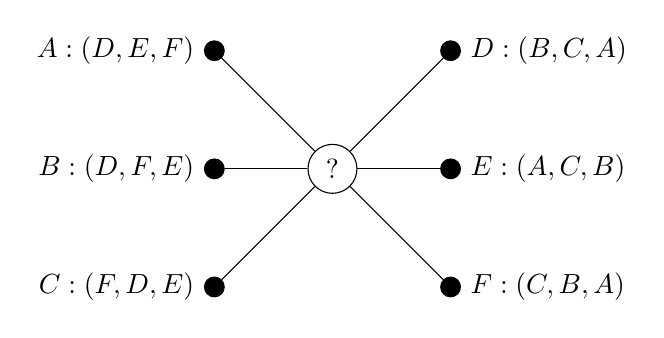
\begin{tikzpicture}[scale=0.5]

        % Suitors
        \node[draw, shape=circle, fill, inner sep=0, minimum size=0.25cm, 
        label=left: {\(A: (D, E, F)\)}] (A) at (0, 0) {};
        \node[draw, shape=circle, fill, inner sep=0, minimum size=0.25cm, 
        label=left: {\(B: (D, F, E)\)}] (B) at (0, -3) {}; 
        \node[draw, shape=circle, fill, inner sep=0, minimum size=0.25cm, 
        label=left: {\(C: (F, D, E)\)}] (C) at (0, -6) {};

        % Reviewers
        \node[draw, shape=circle, fill, inner sep=0, minimum size=0.25cm, 
        label=right: {\(D: (B, C, A)\)}] (D) at (6, 0) {};
        \node[draw, shape=circle, fill, inner sep=0, minimum size=0.25cm, 
        label=right: {\(E: (A, C, B)\)}] (E) at (6, -3)
        {};
        \node[draw, shape=circle, fill, inner sep=0, minimum size=0.25cm,
        label=right: {\(F: (C, B, A)\)}] (F) at (6, -6)
        {};

        % Question mark node
        \node[draw, shape=circle] (q) at (3, -3) {?};
        
        % Lines into (?)
        \foreach \x in {A, B, C, D, E, F}
            \draw (\x) -- (q);

    \end{tikzpicture}
    \caption{A simple matching game represented on a bipartite 
    graph.}\label{fig:matching-bipartite}
    \end{figure}

    Suppose we have the matching shown in Figure~\ref{fig:unstable-matching} for
    our game. This matching, \(M\) is valid since it is a bijection between 
    \(S\) and \(R\) but it is not stable. For instance, we have \((B, D)\) as a
    blocking pair since \(B\) would rather be matched with \(D\) than its 
    current match \(E\), and \(D\) would prefer to be matched with \(B\) than
    its current match \(A\).\\

    \begin{figure}[h]
    \centering
    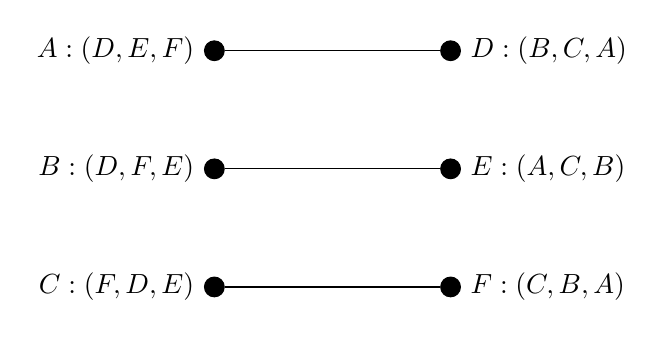
\begin{tikzpicture}[scale=0.5]

        % Suitors
        \node[draw, shape=circle, fill, inner sep=0, minimum size=0.25cm, 
        label=left: {\(A: (D, E, F)\)}] (A) at (0, 0) {};
        \node[draw, shape=circle, fill, inner sep=0, minimum size=0.25cm, 
        label=left: {\(B: (D, F, E)\)}] (B) at (0, -3) {}; 
        \node[draw, shape=circle, fill, inner sep=0, minimum size=0.25cm, 
        label=left: {\(C: (F, D, E)\)}] (C) at (0, -6) {};

        % Reviewers
        \node[draw, shape=circle, fill, inner sep=0, minimum size=0.25cm, 
        label=right: {\(D: (B, C, A)\)}] (D) at (6, 0) {};
        \node[draw, shape=circle, fill, inner sep=0, minimum size=0.25cm, 
        label=right: {\(E: (A, C, B)\)}] (E) at (6, -3)
        {};
        \node[draw, shape=circle, fill, inner sep=0, minimum size=0.25cm,
        label=right: {\(F: (C, B, A)\)}] (F) at (6, -6)
        {};

        % Lines
        \draw (A) -- (D);
        \draw (B) -- (E);
        \draw (C) -- (F);

    \end{tikzpicture}
    \caption{A example of an unstable matching for our game.}\label{%
        fig:unstable-matching}
    \end{figure}

    We can make this matching stable by switching these pairs as in
    Figure~\ref{fig:stable-matching}. Here we have that each suitor is matched 
    with their most preferred reviewer so as not to form a blocking pair. We 
    call such a matching \emph{suitor-optimal}.\\

    \begin{figure}[h]
    \centering
    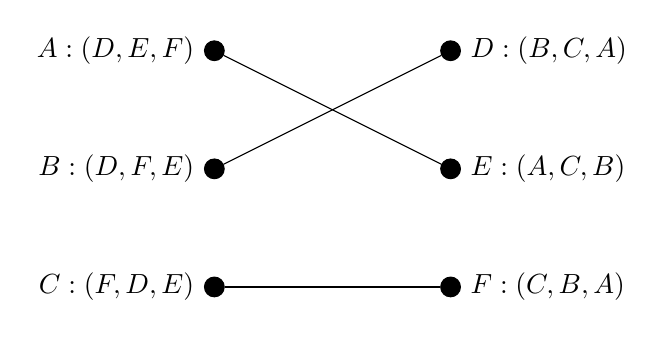
\begin{tikzpicture}[scale=0.5]

        % Suitors
        \node[draw, shape=circle, fill, inner sep=0, minimum size=0.25cm, 
        label=left: {\(A: (D, E, F)\)}] (A) at (0, 0) {};
        \node[draw, shape=circle, fill, inner sep=0, minimum size=0.25cm, 
        label=left: {\(B: (D, F, E)\)}] (B) at (0, -3) {}; 
        \node[draw, shape=circle, fill, inner sep=0, minimum size=0.25cm, 
        label=left: {\(C: (F, D, E)\)}] (C) at (0, -6) {};

        % Reviewers
        \node[draw, shape=circle, fill, inner sep=0, minimum size=0.25cm, 
        label=right: {\(D: (B, C, A)\)}] (D) at (6, 0) {};
        \node[draw, shape=circle, fill, inner sep=0, minimum size=0.25cm, 
        label=right: {\(E: (A, C, B)\)}] (E) at (6, -3)
        {};
        \node[draw, shape=circle, fill, inner sep=0, minimum size=0.25cm,
        label=right: {\(F: (C, B, A)\)}] (F) at (6, -6)
        {};

        % Lines
        \draw (A) -- (E);
        \draw (B) -- (D);
        \draw (C) -- (F);
    \end{tikzpicture}
    \caption{An example of a stable matching for our game.}\label{%
        fig:stable-matching}
    \end{figure}
\end{example}

\subsection{The Gale-Shapley algorithm}\label{subsection:galeshapley}

The Gale-Shapley algorithm is known to find a unique stable matching for any 
matching game of size \(N\). This matching is also considered to be 
suitor-optimal. That is, each suitor is matched with the best possible reviewer
that ensures a stable matching, but is in fact the worst possible matching for 
the reviewers [!!! cite or maybe have these theorems stated/proven !!!]. 

As was discussed at the start of Section~\ref{section:matching}, the outline of
the method proposed in this paper is to extend Huang's method by considering our
virtual modes with some subset of the data as a matching game and then solve it.
It should be noted, however, that in this method we may not have equally sized 
sets of suitors and reviewers. As a result of this, the Gale-Shapley algorithm 
becomes inapplicable as the matching produced \(M\) would not be a bijection of 
our suitors and reviewers.

\subsection{The capacitated Gale-Shapley algorithm for the hospital-resident 
		problem}\label{subsection:capacitated-galeshapley}

The situation where a large set of suitors are to be matched with a number
reviewers is not limited to abstraction. A practical example of this problem is
how to best assign a cohort of medical students to a group of hospitals. Here, 
we have all of the requisite components of a matching game:

\begin{itemize}
	\item A set of reviewers (the hospitals) and a set of suitors (the potential
        residents) 
	\item A ranking of the students/residents by the hospitals, and vice versa
\end{itemize}

The only obstacle which stops us from using the Gale-Shapley algorithm is the 
disparity in the sizes of our sets. In reality, hospitals need not always take 
at most one resident on from a cohort of medical students. So each hospital has
a capacity associated with it and we can consider our matching game to be
`capacitated'. By this we mean that each reviewer may be matched with any number
of suitors up to the capacity associated with them, making our matching \(M: S 
\to R\) surjective. \\

Research surrounding the hospital-resident assignment problem is well-documented 
[cite] and an extension of the Gale-Shapley algorithm was developed to solve it,
awarding the authors the 2012 Nobel Prize in Economic Sciences. This algorithm
is currently used by the National Resident Matching Program 
(\url{http://www.nrmp.org}). \\

As before, we consider a set of suitors and reviewers denoted by \(S\) and 
\(R\). These sets are no longer (necessarily) the same size. We also have our 
preference lists \(f, g\), and a set \(C = \{c_1, \ldots, c_{|R|}\}\) of 
reviewer capacities. Finally, let \(S_u \subset S\) denote the set of suitors 
that are currently unmatched. The capacitated Gale-Shapley algorithm is given 
below.

\begin{algorithm}[H]
\caption{Capacitated Gale-Shapley}\label{alg:cap-galeshapley}
    \begin{algorithmic}[0]
        \For{\(s \in S\)}
            \State{\(M(s) \gets \emptyset\)}
	    \EndFor
        \For{\(r \in R\)}
            \State{\(M^{-1}(r) \gets \emptyset\)}
	    \EndFor
        \State{\(S_u \gets S\)}
        \While{\(|S_u| > 0\)}
            \State{Select any \(s \in S_u\).}
            \If{\(|f(s)| = 0\)}
                \State{\(S_u \gets S_u \setminus \{s\}\)}
		    \Else
                \State{Select \(s\)'s most preferred reviewer \(r \in R\).}
                \If{\(|M(r)| < c_r\)}
                    \State{\(M(r) \gets M(r) \cup \{s\}\)}
                    \State{\(S_u \gets S_u \setminus \{s\}\)}
		        \Else
                    \For{\(s' \in M(r)\)}
                        \If{\(s \notin M(r)\)}
                            \If{\(r\) prefers \(s\) to \(s'\)}
                                \State{\(M(r) \gets M(r) \cup \{s\}\)}
                                \State{\(S_u \gets S_u \cup \{s\}\)}
                                \State{\(M(r) \gets M(r) \setminus \{s'\}\)}
                                \State{\(S_u \gets S_u \cup \{s'\}\)}
				            \Else
                                \State{\(f(s) \gets f(s) \setminus \{r\}\)}
				            \EndIf
			            \EndIf
			        \EndFor
		        \EndIf
		    \EndIf
	    \EndWhile
	\end{algorithmic}
\end{algorithm}

\begin{remark}
	This implementation requires all residents to be ranked by all hospitals, 
    and will produce a matching such that no hospital is left without at least 
    one resident.
\end{remark}




\section{The proposed method}\label{section:new-method}
Now that we have defined what we mean by a matching game, with the algorithm 
described above, we can construct an alternative initialisation process for the 
\(k\)-modes algorithm. \\

Let \textbf{X} be a dataset with attribute set \textbf{A}, and let \(\bar{\mu}\) 
be the set of virtual modes found by Huang's method (i.e.\ the set of centroids 
found in the mode which are to be assigned to points in \textbf{X}). We then 
take this set of virtual modes \(\bar{\mu}\) and construct a capacitated 
matching game to be solved by the capacitated Gale-Shapley algorithm in the 
following way.

\begin{algorithm}[H]
\caption{The proposed initialisation method}
    \begin{algorithmic}[0]
        \State{Find \(\bar{\mu}\) according to Huang's method, up until the 
        final `for' loop.}
        \State{\(R \gets \bar{\mu}\)}
        \State{\(S \gets \emptyset\)}
        \State{\(C \gets \left{1, \ldots, 1\right}\)}
        \For{\(r \in R\)}
            \State{Find the set of \(k\) vectors, \(S_r\), in \textbf{X} that 
            are the least dissimilar to \(r\).}
            \State{\(S \gets S \cup S_r\)}
        \EndFor
        \For{\(r \in R\)}
        \State{\(g(r) \gets S_r\) (here, \(S_r\) is a tuple in descending order
        of similarity)}
        \EndFor
        \State{Select a method for suitor preference lists (see 
        Section~\ref{sec:prefs}) and construct \(f(s)\) accordingly for each \(s
        \in S\).}
        \State{Solve the capacitated matching game defined by \((S, R, C)\) to
        obtain a matching \(M: R \to S\)}.
        \For{\(r in R\)}
            \State{\(\mu^{(l)} \gets M(r)\)}.
        \EndFor
    \end{algorithmic}
\end{algorithm}

\begin{remark}
    The method for constructing the preference lists of our suitors can affect
    the outcome and performance of this method. Please refer to
    Sections~\ref{sec:prefs}~\&~\ref{sec:results}.
\end{remark}



\section{Resident preference lists}\label{section:preferences}
Some examples and hopefully some mathematical reasoning to justify that certain
choices of preference lists reduce down to near equivalent results of the Huang
method (or others). This then suggests the proposed method is in fact a
generalisation of the other method(s).




\section{Experimental results}\label{section:results}
To give comparative results on the quality of the initialisation processes 
defined in
Sections~\ref{sec:init},~\ref{sec:proposed-method}~\&~\ref{sec:preferences},
four well-known, categorical, labelled datasets \- soybean, mushroom, breast
cancer, and zoo animal \- will be clustered with the \(k\)-modes algorithm with
each of the initialisation processes. Rather than comparing our algorithms with
the typical metrics for classification algorithms (accuracy, precision and
recall) the comparison will be based on four clustering performance measures:
adjusted Rand index, adjusted mutual information, homegeneity and completeness.
Definitions of these metrics are given below. In addition to these, we will also
consider the final cost and number of iterations of the best runs for each
initialisation process. As a general rule, each algorithm will be trained on
approximately two thirds of the respective dataset and tested against the final
third.

\subsection{Performance metrics}\label{subsec:metrics}

Usually in the comparison of \(k\)-modes initialisation
processes~\cite{Huang98}\cite{Cao09}, metrics for gauging the quality of
classification algorithms are typically used. As \(k\)-modes is not a
classification algorithm but one for clustering datasets, we will utilise less
class-specific metrics. In their place are metrics built around more general
characteristics of a given clustering. In some respects, however, the metrics
defined below have been considered similar to their classification
counterparts.\\

\begin{definition}\label{def:contingency}
    Let \textbf{X} be a given dataset and consider two clusterings of this
    dataset:
    \[
        U = \left\{U_1, \ldots, U_r\right\}
        \ \text{and} \
        V = \left\{V_1, \ldots, V_s\right\}
    \]

    We do not require that \(r = s\). Now we define a \emph{contingency table},
    denoted by \(\left[n_{ij}\right]\), to summarise the similarity between our
    two clusterings. This table has entries given by
    \(n_{ij}~=~|U_i~\cap~V_j|\), and a representation of this table is shown in
    Table~\ref{tab:contingency}.

    \begin{table}[H]
    \centering
    \begin{tabular}{cccccc}
        {} & \(V_1\) & \(V_2\) & \(\cdots\) & \(V_s\) & Total
        \\ \midrule
        \(U_1\) & \(n_{11}\) & \(n_{12}\) & \(\cdots\) & \(n_{1s}\) & \(a_1\)
        \\
        \(U_2\) & \(n_{21}\) & \(n_{22}\) & \(\cdots\) & \(n_{2s}\) & \(a_2\)
        \\
        \(\vdots\) & \(\vdots\) & \(\vdots\) & \(\ddots\) & \(\vdots\) &
        \(\vdots\)
        \\
        \(U_r\) & \(n_{r1}\) & \(n_{r2}\) & \(\cdots\) & \(n_{rs}\) & \(a_r\)
        \\ \midrule
        Total & \(b_1\) & \(b_2\) & \(\cdots\) & \(b_s\) & {}
    \end{tabular}
    \caption{The contingency table for two clusterings \(U, V\) of a dataset
    \textbf{X}.}\label{tab:contingency}
    \end{table}

    In addition to these entries, we have taken the sums of the each row and of
    each column, and denoted them by \(a\)~and~\(b\), respectively. That is:
    \[
        a_i = \sum_{j=1}^s n_{ij} \ \forall i = 1, \ldots, r, \quad \text{and}
        \quad b_j = \sum_{i=1}^r n_{ij} \ \forall j = 1, \ldots, s
    \]\\
\end{definition}

\begin{definition}\label{def:adjusted-rand-index}
    Let \textbf{X} be a dataset, \(U, V\) be two clusterings of the elements of
    \textbf{X}, and \(\left[n_{ij}\right]\) be the corresponding contingency
    table. Then the adjusted Rand index of these clusterings is given by:
    \[
        ARI(U, V) = \frac{\displaystyle{\sum_{ij} {n_{ij}\choose 2} -
        \frac{1}{{N\choose 2}}\left[\sum_i {a_i\choose 2}\sum_j {b_j\choose
        2}\right]}}{\displaystyle{\frac{1}{2} \left[\sum_i {a_i\choose 2} +
        \sum_j{b_j\choose 2}\right] - \frac{1}{{N\choose 2}}\left[\sum_i
        {a_i\choose 2}\sum_j {b_j\choose 2}\right]}}
    \]\\
\end{definition}

\begin{definition}\label{def:adjusted-mutual-info}
    Let \textbf{X} be a dataset, \(U, V\) be two clusterings of the elements of
    \textbf{X}, and \(\left[n_{ij}\right]\) be the corresponding contingency
    table. Then we define the following quantities:
    \begin{itemize}
        \item Consider a clustering \(C = \left\{C_1, \ldots, C_k\right\}\) of
            \textbf{X}. Then the \emph{entropy}, denoted by \(H(C)\), which is
            associated with this clustering is defined to be:
            \[
                H(C) = - \sum_{i=1}^k P(C_i)\log P(C_i), \quad \text{where}
                \quad P(C_i) = \frac{\left|C_i\right|}{N}
            \]

            \(H(C)\) is non-negative and only takes the value \(0\) when
            \(k~=~1\), i.e.\ there is only one cluster.

        \item Consider our two clusterings \(U, V\). We wish to quantify the
            information shared by both clusterings. This quantity is called the
            \emph{mutual information} between these clusterings, and is defined
            to be:
            \[
                MI(U, V) = \sum_{i=1}^r \sum_{j=1}^s P(U_i, V_j)\log
                \frac{P(U_i, V_j)}{P(U_i)P(V_j)}, \quad \text{where} \quad P(U_i,
                V_j) = \frac{\left|U_i \cap V_j\right|}{N}
            \]

            \(MI(U, V)\) is also non-negative and is bounded from above by
            \(H(U)\) and \(H(V)\).

        \item Using a combinatorial approach (in a similar fashion to
            Definition~\ref{def:adjusted-rand-index}), and a hypergeometric
            model of randomness, we define the
            \emph{expected~mutual~information} of two random clusterings to be:
            \[
                \mathbb{E}\left(MI(U, V)\right) = \sum_{i=1}^r \sum_{j=1}^s
                \sum_{n_{ij}=n_{ij}^*}^{\min(a_i, b_j)} \frac{n_{ij}}{N}\log
                \left(\frac{n_{ij} N}{a_i b_j}\right) \times \frac{a_i!\, b_j!\,
                \left(N - a_i\right)!\, \left(N - b_j\right)!}{N!\, n_{ij}!\,
                \left(a_i - n_{ij}\right)!\, \left(b_j - n_{ij}\right)!\,
                \left(N - a_i - b_j + n_{ij}\right)!}
            \]
            Here, we have \(n_{ij}^* = \max(1, a_i + b_j - N)\).\\
    \end{itemize}
    
    With these quantities, we define the \emph{adjusted mutual information} of
    our pair of clusterings to be:
    \[
        AMI(U, V) = \frac{MI(U, V) - \mathbb{E}\left(MI(U, V)\right)}{\max
        \left(H(U), H(V)\right) - \mathbb{E}\left(MI(U, V)\right)}
    \]
\end{definition}

\begin{remark}
    This adjusted quantity takes values in the interval \(\left[0, 1\right]\).
    In fact, \(AMI(U, V)~=~1\) when \(U\) and \(V\) are indentical, and
    \(AMI(U, V)~=~0\) when the mutual information between the two clusterings is
    equal to the expectation of the mutual information, by chance.\\
\end{remark}

\begin{definition}\label{def:homogeneity}
\end{definition}

\begin{definition}\label{def:completeness}
\end{definition}

\subsection{The datasets}\label{subsec:datasets}

A bit on the structure of each dataset and links to access them.


\subsection{Results}\label{subsec:results}

Tables of results for each dataset and each initialisation process. Credit to 
\url{https://github.com/nicodv/kmodes} for the Python implementation of both the
Huang and Cao processes, as well as the $k$-modes algorithm itself.

\begin{table}[H]
\resizebox{\textwidth}{!}{%
\centering
    \begin{tabular}{llrrrrrr}
\toprule
    &      &  RandIndex &  Mutual Information &  Homogeneity &  Completeness &  Final Cost &  Number of Iterations \\
Initialisation & {} &            &                     &              &               &             &                       \\
\midrule
Cao & mean &   0.732680 &            0.736883 &     0.839891 &      0.833527 &  159.800000 &              2.100000 \\
    & std &   0.176722 &            0.114551 &     0.058968 &      0.090753 &    5.827140 &              0.316228 \\
Huang & mean &   0.673213 &            0.723988 &     0.891716 &      0.810137 &  152.100000 &              2.300000 \\
    & std &   0.149177 &            0.090000 &     0.040811 &      0.069407 &    3.860052 &              0.527046 \\
Random & mean &   0.679415 &            0.718514 &     0.884622 &      0.806282 &  153.800000 &              2.500000 \\
    & std &   0.104628 &            0.060502 &     0.043801 &      0.042463 &    5.337498 &              0.699206 \\
Matching & mean &   0.685331 &            0.727037 &     0.870267 &      0.814538 &  152.900000 &              2.700000 \\
    & std &   0.131183 &            0.075638 &     0.039603 &      0.059881 &    6.092801 &              0.707107 \\
\bottomrule
\end{tabular}

}
\end{table}



\printbibliography

\end{document}
